\section{Results}
\subsection{Frozen held-out comparison}
\ifFinalReportReady
\begin{table*}[t]
\centering\scriptsize
\resizebox{\textwidth}{!}{%
\begin{tabular}{lrrrrrrrrrr}
\toprule
&\multicolumn{3}{c}{Source preservation}&\multicolumn{2}{c}{Global naturalness}&\multicolumn{5}{c}{Target alignment}\\
Model&LPIPS$\downarrow$&DreamSim$\downarrow$&CLIP$\uparrow$&FID$\downarrow$&KID$\downarrow$&PSNR$\uparrow$&SSIM$\uparrow$&M-IoU$\uparrow$&CD$\downarrow$&F-Score$\uparrow$\\
\midrule
Zero-shot, source-only RGB4&0.061884&0.153975&0.943278&36.089871&0.0014905934&22.4062&0.936489&0.814896&0.0167443&0.766221\\
Zero-shot, edited target + source RGB3&0.058324&0.154276&0.942090&35.024202&0.001618189&23.5416&0.945824&0.882545&0.0148793&0.808255\\
Vanilla V1&0.057245&0.151460&0.942854&34.658819&0.0017537581&23.8360&0.946375&0.889032&0.0141140&0.828473\\
Top-1 R&0.056329&0.151162&0.943177&34.930351&0.001822029&23.9966&0.947295&0.898210&0.0136234&0.834758\\
Selected model&0.056201&0.152069&0.943018&34.361368&0.0016011107&24.0283&0.947532&0.901072&0.0136001&0.834532\\
\bottomrule
\end{tabular}}
\caption{Actual frozen TEST508 results from134 source clusters. Source LPIPS/DreamSim/CLIP average cameras9/10; target PSNR/SSIM/2D mask IoU use camera8. Surface CD is symmetric unsquared Euclidean distance; F-Score uses threshold0.02 in the common normalized frame. Official Inception2048 FID/KID use the same1524-image prediction/reference pools. KID is signed and shown in raw units, without clipping or rescaling. References use original materials on edited M1 geometry. These are input-camera evaluations. The selected physical model is SELECTED; a merged baseline is not repeated as another model.}
\label{tab:final-main}
\end{table*}

Table~\ref{tab:final-main} reports the complete frozen five-pipeline
comparison plus the added single-view reference on 508 TEST objects and 134
source clusters. The added RGB1 row has the highest target input-camera
PSNR/SSIM/mask IoU points (24.543 dB/0.95139/0.92725), but its surface CD
and F-Score (0.01789/0.74311) are worse than the four-view edited zero-shot
and selected models. Its source LPIPS/DreamSim/CLIP are
0.06090/0.16202/0.94062, versus 0.05620/0.15207/0.94302 for the selected
model. Original single-view denoisers and native guidance differ from the
multi-view controls, so these descriptive differences cannot be attributed
to view count alone. Within the frozen five-model family, supplying the edited
target RGB changes the zero-shot target PSNR from 22.406 to 23.542 dB,
mask IoU from 0.8149 to 0.8825, CD from 0.01674 to 0.01488, and surface
F-Score from 0.7662 to 0.8083. Vanilla fine-tuning reaches 23.836 dB,
0.8890, 0.01411, and 0.8285, respectively. These zero-shot and vanilla
comparisons are descriptive; the predeclared adjusted family tests the
selected pipeline against the two fine-tuned controls. The different
zero-shot inputs separate access to edited RGB evidence from the subsequent
fine-tuning comparison, without treating input availability as a learned
module effect.

The selected Fixed-SS/Top-1-R-PBR composition has source LPIPS 0.05620 and
target PSNR 24.028 dB, SSIM 0.94753, and mask IoU 0.90107. Relative to
vanilla V1, the paired differences are $-0.001044$, $+0.1923$ dB,
$+0.001156$, and $+0.012041$. Their 16-endpoint family-adjusted 95\%
intervals exclude zero (Supplementary
Table~\ref{tab:final-adjusted-contrasts}). The selected pipeline has a
lower CD point estimate (0.01360 versus 0.01411) and a higher surface
F-Score (0.83453 versus 0.82847), but the adjusted intervals for both
contain zero. Source DreamSim is 0.15207 versus V1's 0.15146, and its
adjusted interval also contains zero; the same is true for source CLIP.
Thus the held-out support is endpoint-specific, rather than a claim that
geometry and source appearance improve on every measure.

Against the Top-1 retargeting baseline, the selected pipeline has small
favorable points for LPIPS, target PSNR, SSIM, mask IoU, and CD, but a
higher (worse) DreamSim and slightly lower F-Score. Every one of the eight
predeclared adjusted intervals contains zero. This comparison does not
establish that the selected Top-K weighted SS path contributes additional
held-out quality beyond the retargeting baseline, nor does it establish
equivalence. The added single-view baseline has the lowest FID point (34.147),
while the source-only four-view zero-shot model has the lowest KID point
(0.001491). FID
and signed raw KID summarize common 1,524-image input-camera pools and are
descriptive, without a paired significance claim.

\else
The five-model TEST508 cascade and ten-metric evaluation are in progress.
The final Main table will be imported from the closed source-bound collector;
development means are not substituted into it. The comparison separates the
information supplied by an edited target from the effect of fine-tuning and
retargeting. Its geometric and appearance findings remain unasserted here.
\fi

\subsection{Geometric component comparisons}
\input{typeset/final-ablation-template.tex}
All seven SS designs have completed 480 updates, DEV128 three-noise
diagnostics, and actual surface evaluation under common downstream models.
Spatial, raw semantic, decoder-cosine and scalar Fixed give CD 0.0129704,
0.0128789,0.0128065 and 0.0127572, with F-Score 0.839333,0.841031,0.842414
and 0.844058. The point-estimate ladder improves both geometric endpoints,
but every interval in the 48-comparison family includes zero.

Fixed minus Top-1 changes F-Score by 0.003963, with adjusted
interval $[-0.000910,0.009748]$; Fixed minus Uniform gives 0.001553 with
$[-0.003326,0.007439]$; physical retargeter removal gives a Fixed advantage
of 0.009020 with $[-0.001582,0.020293]$. CD intervals also contain zero.
We select Fixed by the lowest CD/highest F-Score points, while retaining
uncertainty about component effects. Spatial 3 versus semantic 64 is a
module substitution, Top-1 versus weighted Top-K bundles candidate count
and aggregation, and scalar matching can change support. Uniform on the
same support is the separate weighting control.

\subsection{Appearance on identical selected geometry}
\input{typeset/dev-selected-pbr-appearance32.tex}
The four PBR variants share actual generated Fixed geometry, native guides,
texture noise, triangles and references. Top-1 R has the lowest source
LPIPS/DreamSim points, 0.053290/0.157828, versus vanilla 0.053513/0.158346.
Their exploratory paired deltas are $-0.000223$ with
$[-0.000539,0.000035]$ and $-0.000517$ with $[-0.002250,0.001183]$.
Both intervals include zero. Feature/Raw variants do not improve either
primary point over Top-1 R; vanilla has the best complementary CLIP point.
We choose the measured Top-1 R PBR and report target image metrics separately.
Identical CD/F-Score confirm geometry equality, not a PBR geometry gain.
The feature/Raw arms retain a Top-1 carrier/use path and do not establish the
effect of a shared Fixed PBR pathway.

\subsection{Retrieval evidence and generated quality}
Decoder matching improves exact rank-one coverage from 1.25\% to 7.73\%
in the separate DEV32 diagnostic. Member proposals raise exact@64 coverage
from 50.76\% to 73.36\%. Native evidence-use analysis finds 31,408 observable
Top-1-miss/Top-K-hit relations; Fixed places more probability on GT proposals
than post-hoc Uniform. These measurements establish available evidence and
its allocation, not a generated-quality improvement. The original learned
ray-versus-voxel and member-versus-mean studies do not establish positive
quality effects; their scope differs from the selected identity-value path.
Full diagnostics and the actual annotated example are in the Supplement.

\subsection{Prespecified qualitative comparison}
\ifFinalReportReady
\begin{figure*}[!t]
\centering
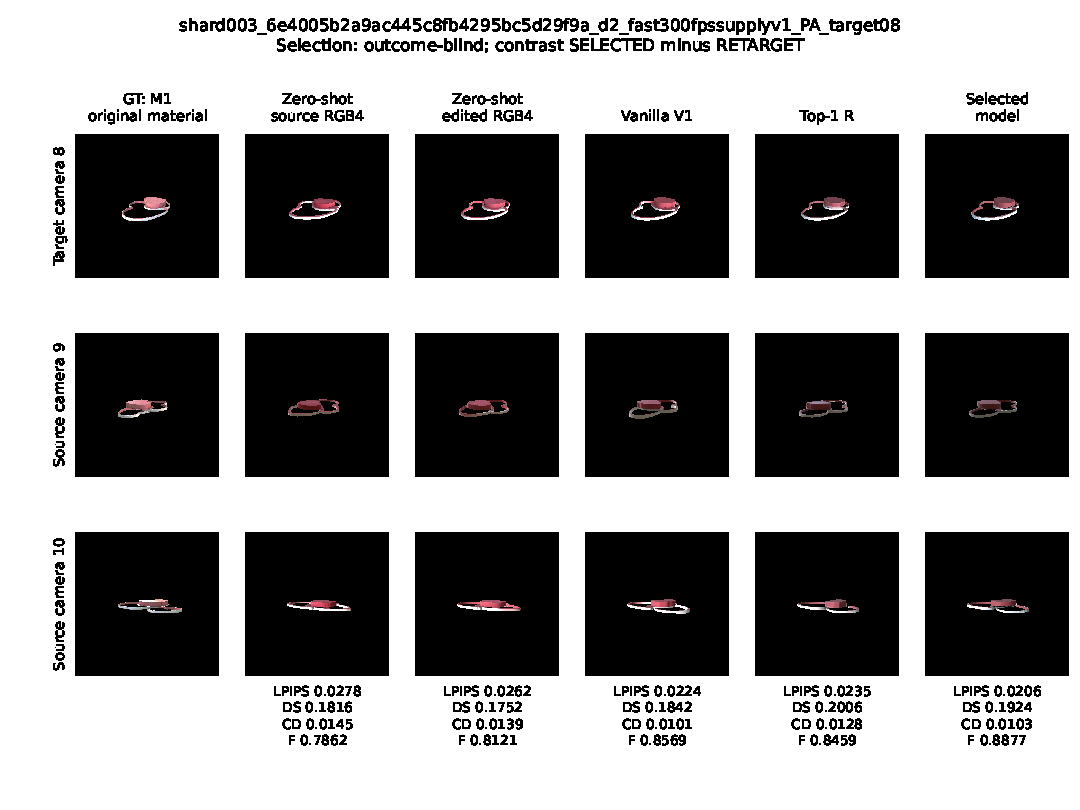
\includegraphics[width=\textwidth]{final-results/figures/example-01.pdf}
\caption{Actual scored frozen TEST example. Rows are target8/source9/source10; columns are the common original-material M1 reference and every frozen model. Selection: outcome-blind. Full-frame panels use the scored archive and official uint8 conversion, without model-specific crop, alignment or rerender. Source annotations use cameras9/10. Conditional categories illustrate their stated conditions and do not estimate population success rates.}
\label{fig:final-qualitative-01}
\end{figure*}

\else
The Main figure is reserved for the first outcome-blind example in the
original metadata declaration. The second outcome-blind example and every
conditional lower-median panel remain in the Supplement. This placement is
fixed before viewing the final panels and is independent of their quality.
The actual scored target/source images will be imported after ten-metric
completion; no placeholder image is presented as an experiment.
\fi
